
\documentclass[notheorems,serif]{beamer}

%选用主题
%\usetheme{Rochester}
%\usetheme{default}
%\usetheme{AnnArbor}
%\usetheme{Antibes}
%\usetheme{Bergen}
%\usetheme{Berkeley}
%\usetheme{Berlin}
%\usetheme{Boadilla}
%\usetheme{CambridgeUS}
%\usetheme{Copenhagen}
%\usetheme{Darmstadt}
%\usetheme{Dresden}
%\usetheme{Frankfurt}
%\usetheme{Goettingen}%
%\usetheme{Hannover}
%\usetheme{Ilmenau}
%\usetheme{JuanLesPins}
%\usetheme{Luebeck}
\usetheme{Madrid}
%\usetheme{Malmoe}
%\usetheme{Marburg}
%\usetheme{Montpellier}
%\usetheme{PaloAlto}
%\usetheme{Pittsburgh}
%\usetheme{Rochester}
%\usetheme{Singapore}
%\usetheme{Szeged}
%\usetheme{Warsaw}

% As well as themes, the Beamer class has a number of color themes
% for any slide theme. Uncomment each of these in turn to see how it
% changes the colors of your current slide theme.

%\usecolortheme{albatross}
%\usecolortheme{beaver}
%\usecolortheme{beetle}
%\usecolortheme{crane}
%\usecolortheme{dolphin}
%\usecolortheme{dove}
%\usecolortheme{fly}
%\usecolortheme{lily}
%\usecolortheme{orchid}
%\usecolortheme{rose}
%\usecolortheme{seagull}
%\usecolortheme{seahorse}
%\usecolortheme{whale}
%\usecolortheme{wolverine}

%设置被cover的内容不显示
%\setbeamercovered{transparent}

\useinnertheme{rounded}
\usecolortheme{default}

%调用包
\usepackage[no-math, cm-default]{fontspec}
\usepackage{xltxtra}
\usepackage{xunicode}   
\usepackage{xcolor}
\usepackage{amsmath,amssymb}
\usepackage{xeCJK}
\usepackage{multimedia}
\usepackage{listings}
\usepackage{subfigure}
\usepackage{todonotes}
\presetkeys{todonotes}{inline}{} 
\usepackage{multicol}
\usepackage{changes}




%将系统字体名映射为逻辑字体名称,主要是为了维护的方便  
\newcommand\fnhei{Adobe 黑体 Std}  
\newcommand\fnsong{Adobe 宋体 Std}  
\newcommand\fnkai{Adobe 楷体 Std}  
\newcommand\fnmono{DejaVu Sans Mono}  
\newcommand\fnroman{Times New Roman}  

\renewcommand{\normalsize}{\wuhao}

%%设置常用中文字号,方便调用  
\newcommand{\erhao}{\fontsize{22pt}{\baselineskip}\selectfont}  
\newcommand{\xiaoerhao}{\fontsize{18pt}{\baselineskip}\selectfont}  
\newcommand{\sanhao}{\fontsize{16pt}{\baselineskip}\selectfont}  
\newcommand{\xiaosanhao}{\fontsize{15pt}{\baselineskip}\selectfont}  
\newcommand{\sihao}{\fontsize{14pt}{\baselineskip}\selectfont}  
\newcommand{\xiaosihao}{\fontsize{12pt}{\baselineskip}\selectfont}  
\newcommand{\wuhao}{\fontsize{10.5pt}{\baselineskip}\selectfont}  
\newcommand{\xiaowuhao}{\fontsize{9pt}{\baselineskip}\selectfont}  
\newcommand{\liuhao}{\fontsize{7.5pt}{\baselineskip}\selectfont}  


%楷体  
%\newfontinstance\KAI{\fnkai}  
%\newcommand{\kai}[1]{{\KAI#1}}  
%黑体  
%\newfontinstance\HEI{\fnhei}  
%\newcommand{\hei}[1]{{\HEI#1}}  
%英文  
%\newfontinstance\ENF{\fnroman}  
%\newcommand{\en}[1]{\,{\ENF#1}\,}



%连字符
\defaultfontfeatures{Mapping=tex-text}


%%%% 定理类环境的定义 %%%%
\newtheorem{example}{\hei{例子}} 
\newtheorem{problem}{\hei{问题}}           
\newtheorem{algorithm}{\hei{算法}}
\newtheorem{theorem}{\hei{定理}}
\newtheorem{definition}{\hei{定义}}
\newtheorem{axiom}{\hei{公理}}
\newtheorem{property}{\hei{性质}}
\newtheorem{proposition}{\hei{命题}}
\newtheorem{lemma}{\hei{引理}}
\newtheorem{corollary}{\hei{推论}}
\newtheorem{remark}{\hei{注解}}
\newtheorem{condition}{\hei{条件}}
\newtheorem{conclusion}{\hei{结论}}
\newtheorem{assumption}{\hei{假设}}

%重定义一些环境的名字
\renewcommand{\proofname}{\hei{证明}}
\renewcommand\tablename{\hei{表}}

%---SCRIPT-----------------------------------------------------------------------------------------
\newcommand{\cA}{\mathcal{A}}
\newcommand{\cB}{\mathcal{B}}
\newcommand{\cC}{\mathcal{C}}
\newcommand{\cD}{\mathcal{D}}
\newcommand{\cE}{\mathcal{E}}
\newcommand{\ce}{\mathcal{e}}
\newcommand{\cF}{\mathcal{F}}
\newcommand{\cG}{\mathcal{G}}
\newcommand{\cg}{\mathcal{g}}
\newcommand{\cH}{\mathcal{H}}
\newcommand{\cI}{\mathcal{I}}
\newcommand{\cJ}{\mathcal{J}}
\newcommand{\cK}{\mathcal{K}}
\newcommand{\cL}{\mathcal{L}}
\newcommand{\cM}{\mathcal{M}}
\newcommand{\cN}{\mathcal{N}}
\newcommand{\cO}{\mathcal{O}}
\newcommand{\cP}{\mathcal{P}}
\newcommand{\cQ}{\mathcal{Q}}
\newcommand{\cR}{\mathcal{R}}
\newcommand{\cS}{\mathcal{S}}
\newcommand{\cT}{\mathcal{T}}
\newcommand{\cU}{\mathcal{U}}
\newcommand{\cV}{\mathcal{V}}
\newcommand{\cW}{\mathcal{W}}
\newcommand{\cX}{\mathcal{X}}
\newcommand{\cY}{\mathcal{Y}}
\newcommand{\cZ}{\mathcal{Z}}
\newcommand{\cz}{\mathcal{z}}
%---BLACKBOARD-------------------------------------------------------------------------------------
\newcommand{\mA}{\mathbb A}
\newcommand{\mB}{\mathbb B}
\newcommand{\mC}{\mathbb C}
\newcommand{\mD}{\mathbb D}
\newcommand{\mE}{\mathbb E}
\newcommand{\mF}{\mathbb F}
\newcommand{\mG}{\mathbb G}
\newcommand{\mg}{\mathbb g}
\newcommand{\mH}{\mathbb H}
\newcommand{\mI}{\mathbb I}
\newcommand{\mJ}{\mathbb J}
\newcommand{\mK}{\mathbb K}
\newcommand{\mL}{\mathbb L}
\newcommand{\mM}{\mathbb M}
\newcommand{\mN}{\mathbb N}
\newcommand{\mO}{\mathbb O}
\newcommand{\mP}{\mathbb P}
\newcommand{\mQ}{\mathbb Q}
\newcommand{\mR}{\mathbb R}
\newcommand{\mS}{\mathbb S}
\newcommand{\mT}{\mathbb T}
\newcommand{\mU}{\mathbb U}
\newcommand{\mV}{\mathbb V}
\newcommand{\mW}{\mathbb W}
\newcommand{\mX}{\mathbb X}
\newcommand{\mY}{\mathbb Y}
\newcommand{\mZ}{\mathbb Z}
\newcommand{\mz}{\mathbb z}

\newcommand{\bV}{\mathbf{V}}
\newcommand{\bz}{\mathbf{z}}
\newcommand{\bT}{\mathbf{T}}
\newcommand{\bx}{\mathbf{x}}
\newcommand{\be}{\mathbf{e}}
\newcommand{\bff}{\mathbf{f}}
\newcommand{\bg}{\mathbf{g}}
\newcommand{\bn}{\mathbf{n}}
\newcommand{\bt}{\mathbf{t}}
\newcommand{\bd}{\mathbf{d}}
\newcommand{\bzero}{\mathbf{0}}
\newcommand{\bka}{\mathbf{\kappa}}

\newcommand{\rd}{\mathrm{d}}
%---SHORTCUTS--------------------------------------------------------------------------------------
\newcommand\xor{\mathbin{\char`\^}}
\DeclareMathOperator{\res}{Res}
\DeclareMathOperator{\sgn}{sgn}
\DeclareMathOperator{\supp}{supp}
\DeclareMathOperator{\as}{as}
\newcommand{\slant}[1]{\slshape #1\normalfont}
\newcommand{\dd}[2]{\frac{d#1}{d#2}} 
\newcommand{\ddx}{\frac{d}{dx}}
\newcommand{\ddt}{\frac{d}{dt}}
\newcommand{\dds}{\frac{d}{ds}}
\newcommand{\pd}[1]{\ds\frac{\partial}{\partial #1 }}
\newcommand{\pdd}[2]{\ds\frac{\partial #1}{\partial #2 }}
\newcommand{\mdd}[3]{\ds\frac{\partial^{#3} #1}{\partial #2^{#3} }}
\newcommand{\x}{\ _\Box}
\newcommand{\ds}{\displaystyle}
\newcommand{\bs}{\backslash}
\newcommand{\Bold}{\noindent \bfseries}
\newcommand{\Norm}{\normalfont}
\newcommand{\exl}[1]{\textcolor{NavyBlue}{\Bold Exercise #1 \Norm}}
\newcommand{\ex}{\textcolor{NavyBlue}{\Bold Problem: \Norm}}
\newcommand{\sol}{\textcolor{Mulberry}{\Bold Solution: \Norm}}
\newcommand{\pf}{\textcolor{Mulberry}{\Bold Proof: \Norm}}
\newcommand{\Title}[1]{\LARGE\Bold \textcolor{Sepia}{#1}\Norm\normalsize \vspace{10pt} \newline}
\newcommand{\prop}{\Bold \textcolor{YellowOrange}{ Proposition:} \Norm}
\newcommand{\propl}[1]{\Bold \textcolor{YellowOrange}{ Proposition #1:} \Norm}
\newcommand{\rk}{\Bold \textcolor{YellowOrange}{ Remark:} \Norm}
\newcommand{\rmk}[1]{\Bold\textcolor{YellowOrange}{#1} \Norm}
\newcommand{\thm}[1]{\Bold \textcolor{YellowOrange}{ Theorem #1} \Norm}
\newcommand{\ind}{\indent\indent}
\newcommand{\br}{\vspace{10pt} \newline}

\newcommand{\red}{\color{red}}
\newcommand{\blue}{\color{blue}}



\begin{document}

\title[Linux基础和vim]{{\small\leftline{湘潭大学}~~~~~~~~~~~~~~~~~~~~~~~~~~~~~~~~~~~~~~~~~~~~~~
~~~~~~~~~~~} \\
Linux基础和vim
}




\author[]{~~讲课:~~季俊豪~~ \\
\vspace{0.2cm}~专~~~~业:~~数据科学与大数据技术~~}

\institute[湘潭大学数学与计算科学学院]

\date[\today]


\frame[plain]{\titlepage}




\AtBeginSection[]{

  \frame<beamer>{ 

    \frametitle{内容纲要}   

    \tableofcontents[currentsection] 

  }
}


\section{Windows vs Linux}

\begin{frame}
\frametitle{Windows版本}
\begin{itemize}
\item Windows XP
\item Windows 7
\item Windows 8
\item Windows 10
\end{itemize}
\end{frame}

\begin{frame}
\frametitle{Linux版本}
\begin{itemize}
\item Ubuntu 家庭用途
\item CentOS 商用
\item Debian 商用
\item Kali linux 渗透
\end{itemize}
\end{frame}

\begin{frame}
\frametitle{Linux优势}
\begin{itemize}
\item 开源、免费
\item 跨平台的硬件支持
\item 丰富的软件支持,没有华丽花哨的游戏
\item 多用户多任务
\item 可靠的安全性
\end{itemize}
\end{frame}



\section{系统安装}
\subsection{两种方式}
\begin{frame}
\frametitle{虚拟机 or 双系统}
\begin{itemize}
\item 虚拟机\(Virtual Machine\)指通过软件模拟的具有完整硬件系统功能的、运行在一个完全隔离环境中的完整计算机系统。
\item 双系统在安装的时候,两个系统是分别装在不同的分区内,后安装的系统不会覆盖前一个系统。
\end{itemize}
\end{frame}

\subsection{虚拟机安装}
\begin{frame}
\frametitle{虚拟机安装}
双击安装文件VMware-workstation-full-15.5.6-16341506.exe,进入安装欢迎界面,点击下一步
\begin{figure}
%\small
\centering
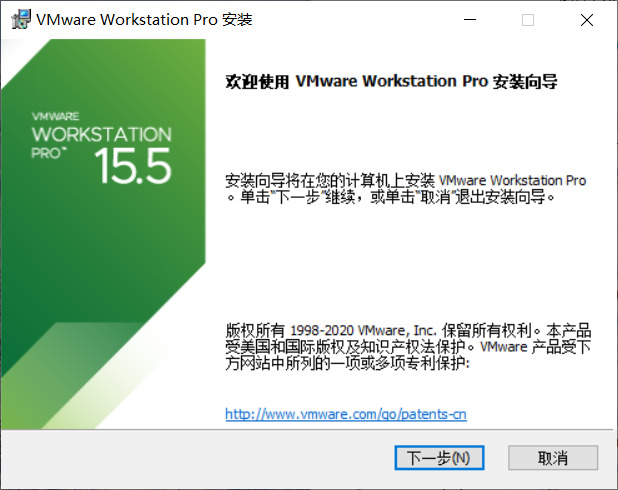
\includegraphics[width=8cm,height=6cm]{./figures/图片1.png}
\end{figure}
\end{frame}

\begin{frame}
\frametitle{虚拟机安装}
在欢迎界面,点击【下一步(N)】按钮后弹出许可协议界面,勾选接受协议条款,点击【下一步(N)】按钮
\begin{figure}
%\small
\centering
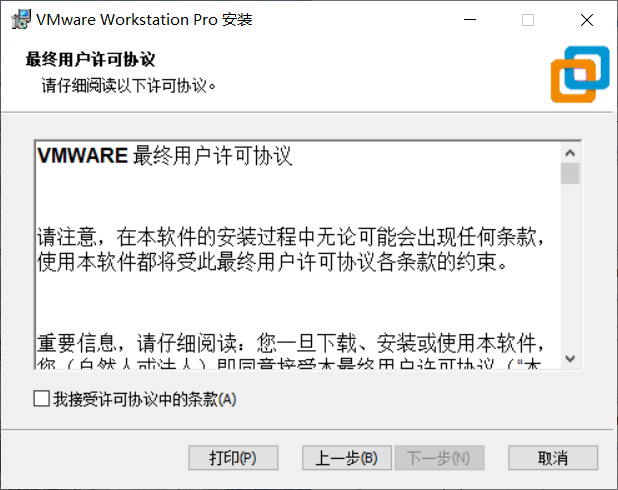
\includegraphics[width=8cm,height=6cm]{./figures/图片2.png}
\end{figure}
\end{frame}

\begin{frame}
\frametitle{虚拟机安装}
进入VMware Workstation安装位置配置界面,可以更改软件安装位置,点击【下一步(N)】按钮
\begin{figure}
%\small
\centering
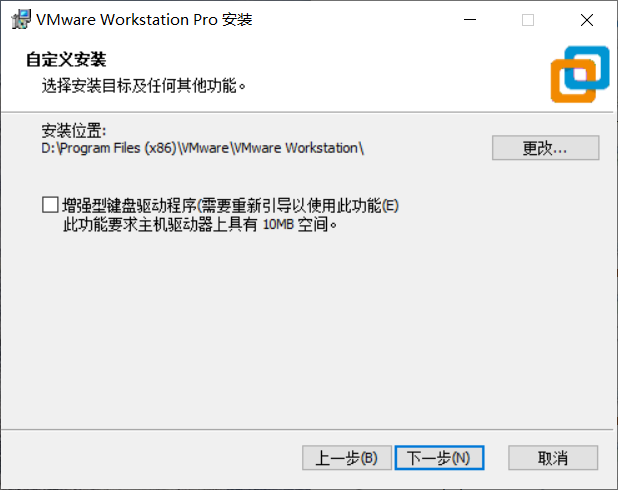
\includegraphics[width=8cm,height=6cm]{./figures/图片3.png}
\end{figure}
\end{frame}

\begin{frame}
\frametitle{虚拟机安装}
进入更新和用户体验改进计划设置界面,默认是勾选的,可以去掉,点击【下一步(N)】按钮
\begin{figure}
%\small
\centering
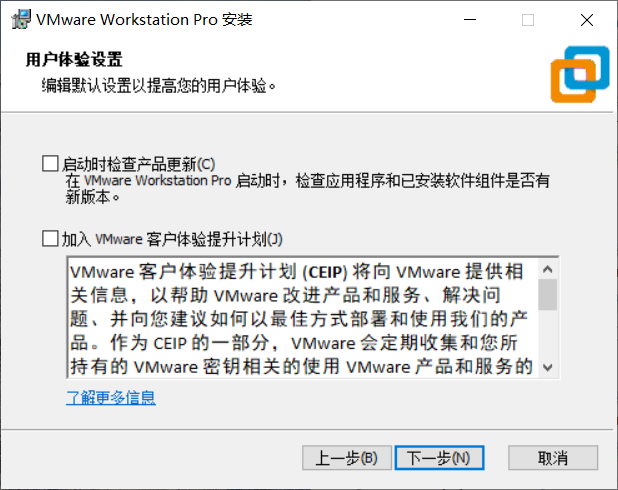
\includegraphics[width=8cm,height=6cm]{./figures/图片4.png}
\end{figure}
\end{frame}

\begin{frame}
\frametitle{虚拟机安装}
进入软件安装后的启动快捷方式设置界面,点击【下一步(N)】按钮
\begin{figure}
%\small
\centering
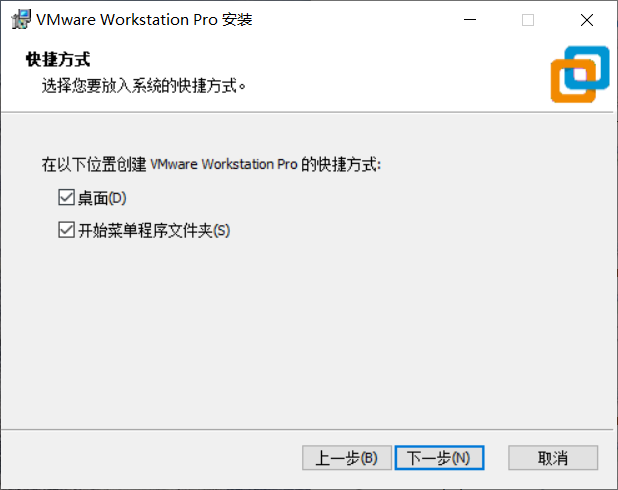
\includegraphics[width=8cm,height=6cm]{./figures/图片5.png}
\end{figure}
\end{frame}

\begin{frame}
\frametitle{虚拟机安装}
点击【安装(I)】,软件开始安装
\begin{figure}
%\small
\centering
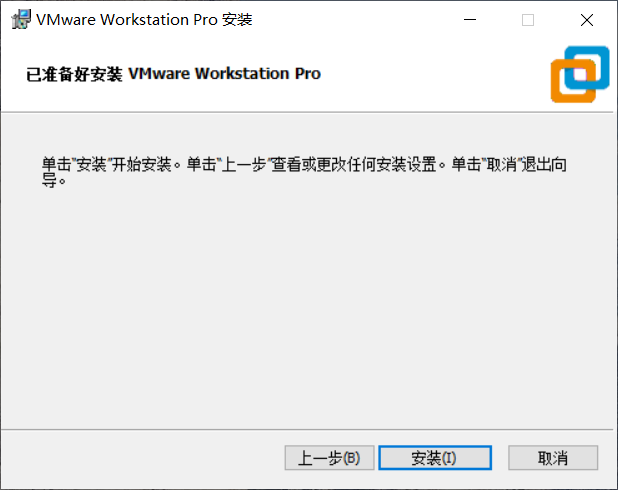
\includegraphics[width=8cm,height=6cm]{./figures/图片6.png}
\end{figure}
\end{frame}

\begin{frame}
\frametitle{虚拟机安装}
 安装完成后打开虚拟机,弹出许可证密钥输入界面,输入秘钥UY758-0RXEQ-M81WP-8ZM7Z-Y3HDA,完成认证
\begin{figure}
 %\small
 \centering
 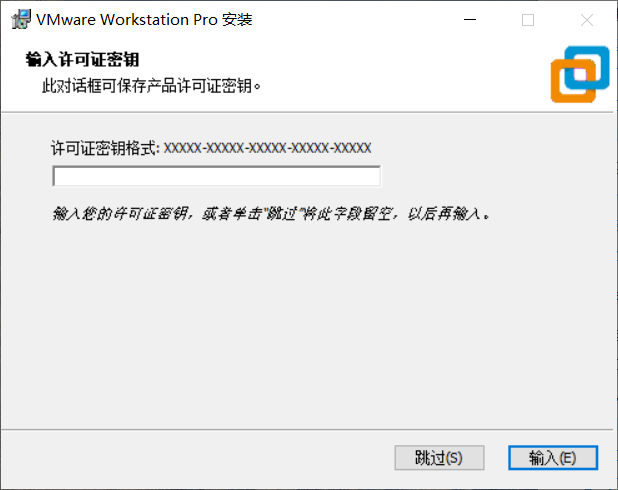
\includegraphics[width=8cm,height=6cm]{./figures/图片7.png}
\end{figure}
\end{frame}

\begin{frame}
\frametitle{虚拟机安装完成}
 打开虚拟机
\begin{figure}
 %\small
 \centering
 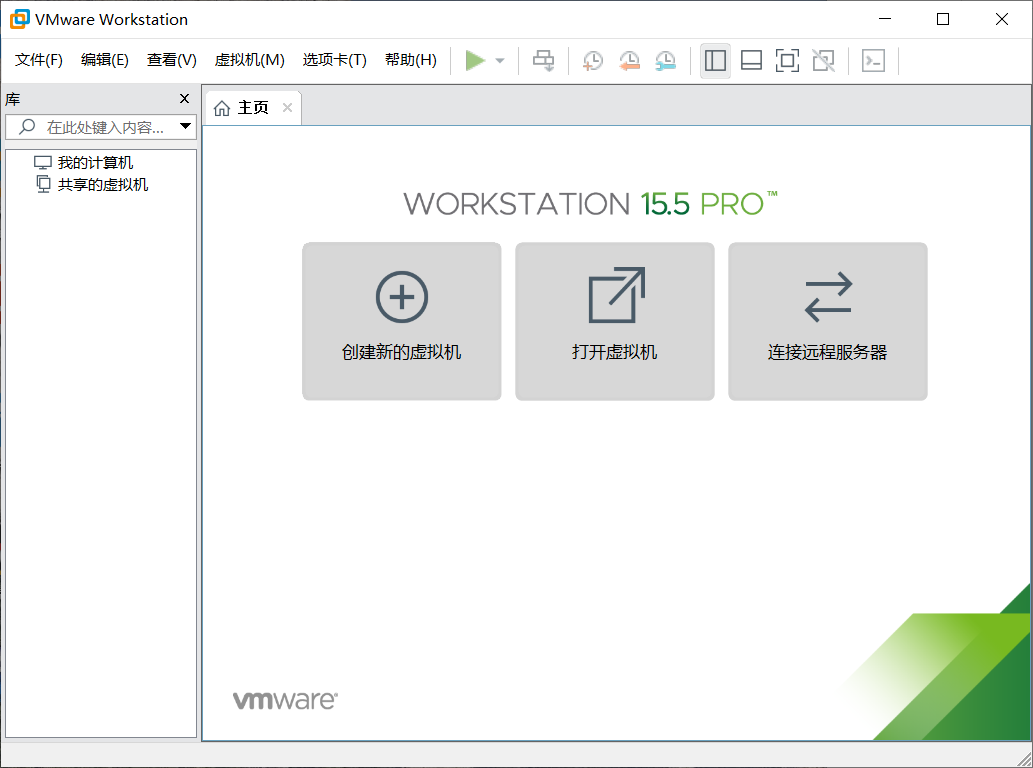
\includegraphics[width=8cm,height=6cm]{./figures/图片8.png}
\end{figure}
\end{frame}


\begin{frame}
\frametitle{系统安装}
点击【创建新的虚拟机】后,进入新建虚拟机向导页面,选择自定义安装,然后点击【下一步(N)】按钮
\begin{figure}
%\small
\centering
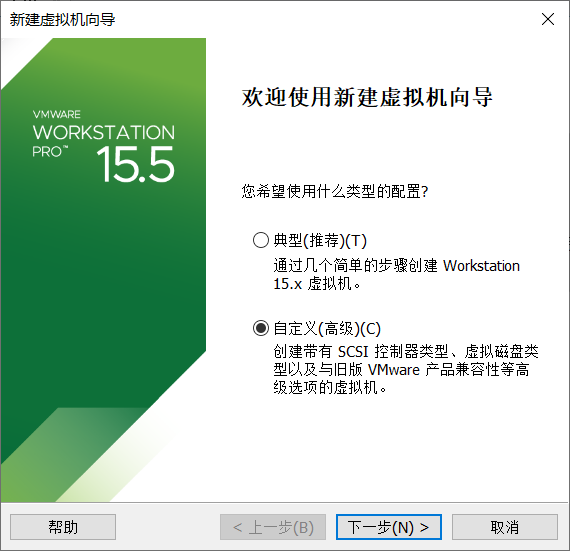
\includegraphics[width=8cm,height=6cm]{./figures/图片9.png}
\end{figure}
\end{frame}

\begin{frame}
\frametitle{系统安装}
进入选择虚拟机硬件兼容性的页面,查看限制信息,点击【下一步(N)】按钮
\begin{figure}
%\small
\centering
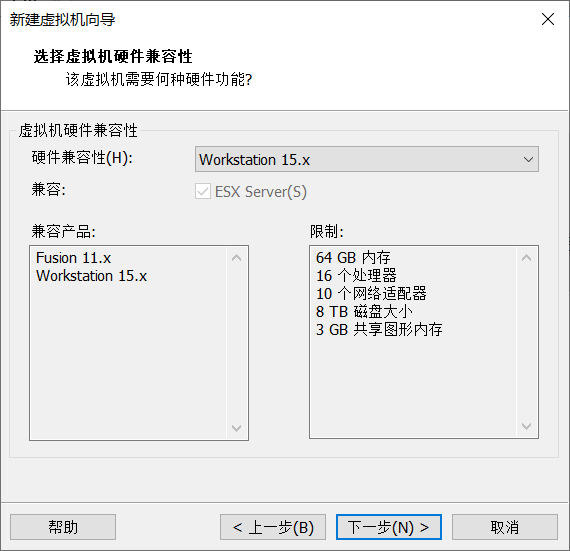
\includegraphics[width=8cm,height=6cm]{./figures/图片10.png}
\end{figure}
\end{frame}

\begin{frame}
\frametitle{系统安装}
进入客户机安装来源页面,选择稍后安装操作系统,然后点击【下一步(N)】按钮
\begin{figure}
%\small
\centering
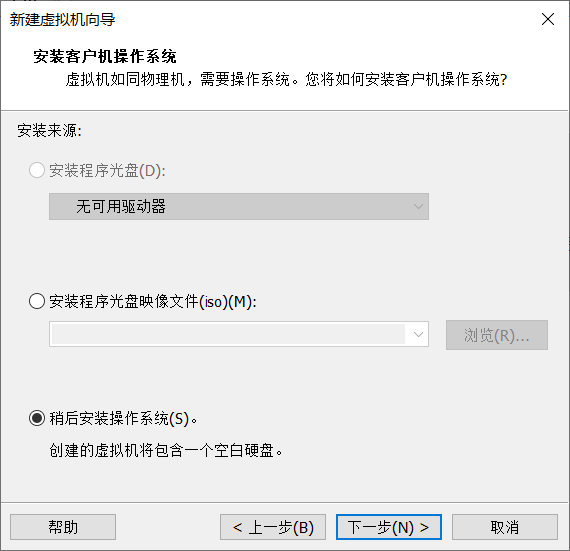
\includegraphics[width=8cm,height=6cm]{./figures/图片11.png}
\end{figure}
\end{frame}

\begin{frame}
\frametitle{系统安装}
进入选择客户机操作系统页面,选择操作系统版本,然后点击【下一步(N)】按钮
\begin{figure}
%\small
\centering
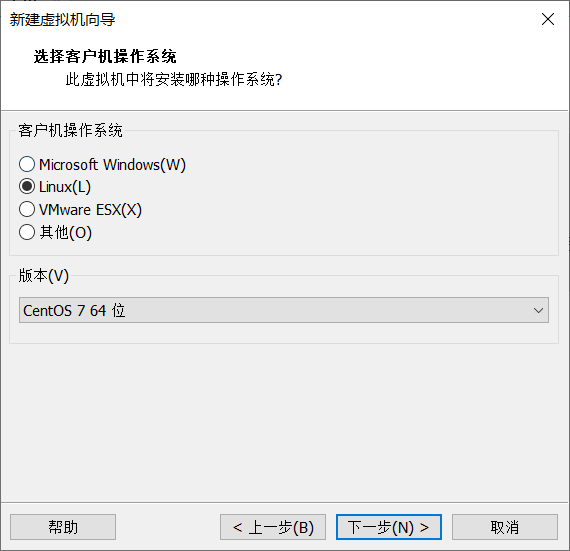
\includegraphics[width=8cm,height=6cm]{./figures/图片12.png}
\end{figure}
\end{frame}

\begin{frame}
\frametitle{系统安装}
进入虚拟机命名页面,输入虚拟机名称,建议起有意义的名称,然后选择镜像文件存放的位置,点击【下一步(N)】按钮
\begin{figure}
%\small
\centering
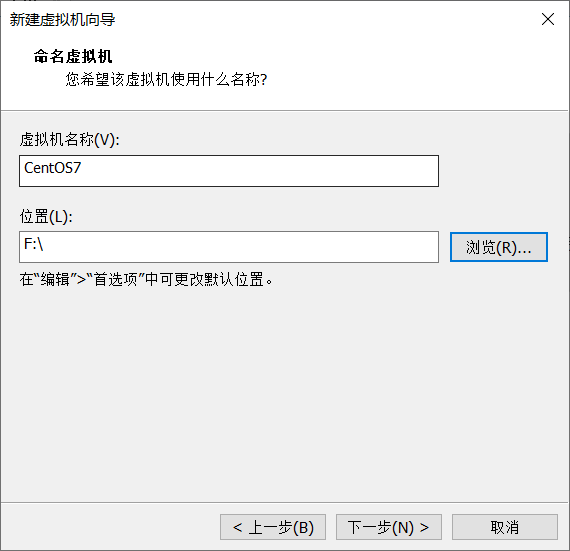
\includegraphics[width=8cm,height=6cm]{./figures/图片13.png}
\end{figure}
\end{frame}

\begin{frame}
\frametitle{系统安装}
进入处理器配置页面,选择给虚拟机分配的cpu核的数量,这里建议修改为双核,然后点击【下一步(N)】按钮
\begin{figure}
%\small
\centering
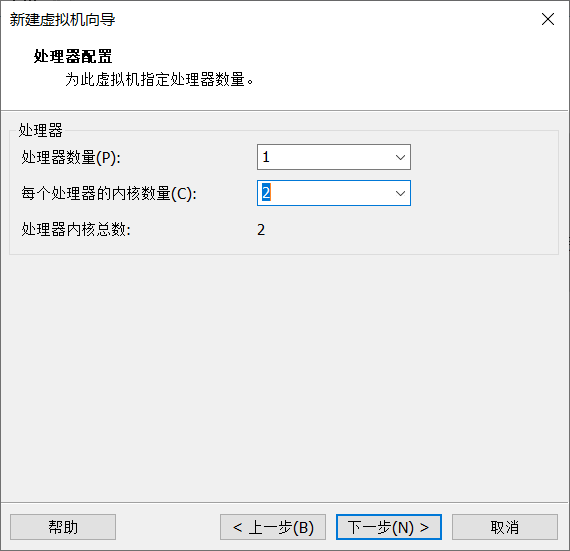
\includegraphics[width=8cm,height=6cm]{./figures/图片14.png}
\end{figure}
\end{frame}

\begin{frame}
\frametitle{系统安装}
进入虚拟机内存分配页面,建议选择2048MB,然后点击【下一步(N)】按钮
\begin{figure}
 %\small
 \centering
 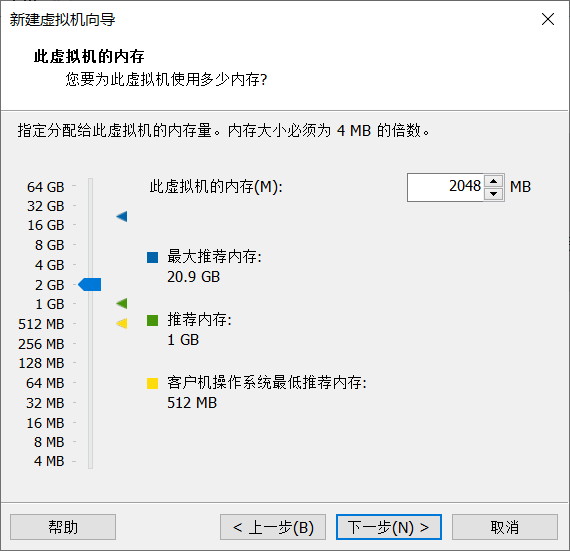
\includegraphics[width=8cm,height=6cm]{./figures/图片15.png}
\end{figure}
\end{frame}

\begin{frame}
\frametitle{系统安装}
进入添加网络类型页面,选择【使用网络地址转换(NAT)(E)】,点击【下一步(N)】按钮
\begin{figure}
 %\small
 \centering
 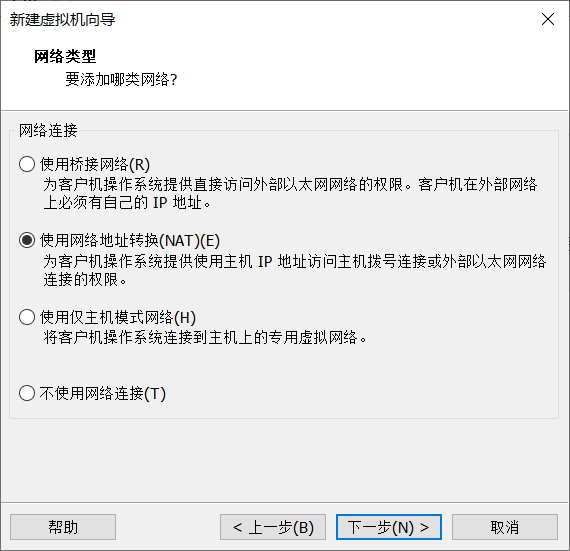
\includegraphics[width=8cm,height=6cm]{./figures/图片16.png}
\end{figure}
\end{frame}


\begin{frame}
\frametitle{系统安装}
进入I/O控制器类型选择页面,建议使用推荐设置,点击【下一步(N)】按钮
\begin{figure}
%\small
\centering
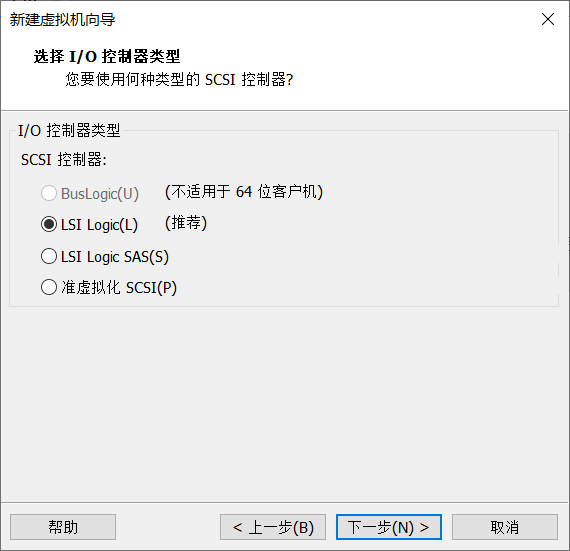
\includegraphics[width=8cm,height=6cm]{./figures/图片17.png}
\end{figure}
\end{frame}

\begin{frame}
\frametitle{系统安装}
进入磁盘类型选择页面,选择要创建的磁盘类型,建议使用推荐设置,点击【下一步(N)】按钮
\begin{figure}
 %\small
 \centering
 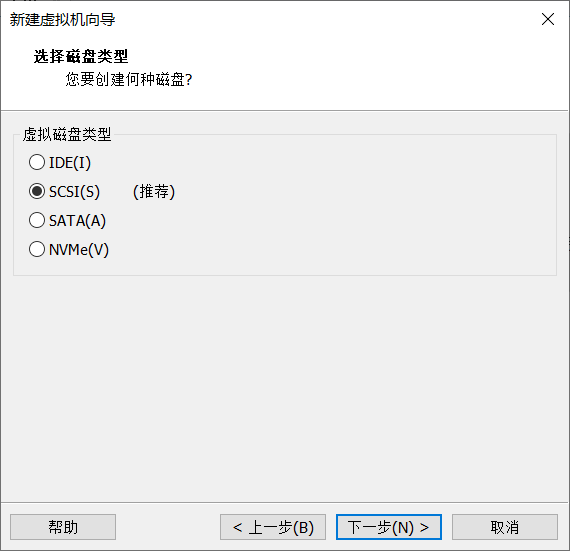
\includegraphics[width=8cm,height=6cm]{./figures/图片18.png}
\end{figure}
\end{frame}

\begin{frame}
\frametitle{系统安装}
进入磁盘选择页面,由于是创建虚拟机,选择创建新虚拟机磁盘选项,点击【下一步(N)】按钮
\begin{figure}
 %\small
 \centering
 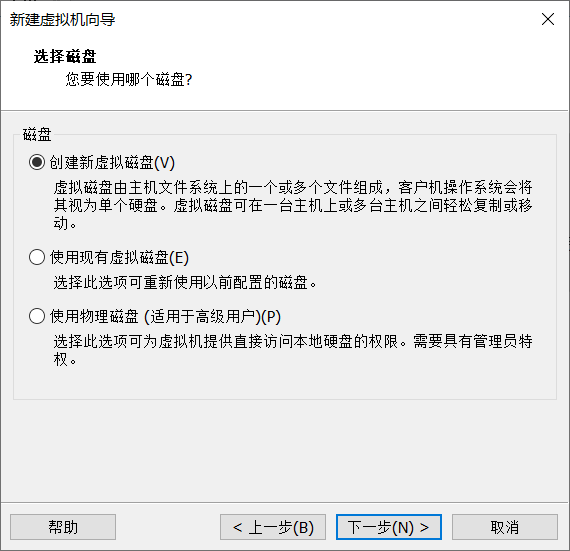
\includegraphics[width=8cm,height=6cm]{./figures/图片19.png}
\end{figure}
\end{frame}

\begin{frame}
\frametitle{系统安装}
进入磁盘容量分配页面,建议【最大磁盘大小(GB)】为30.0GB,并且勾选中【将虚拟磁盘存储为单个文件(O)】,点击【下一步(N)】按钮
\begin{figure}
%\small
\centering
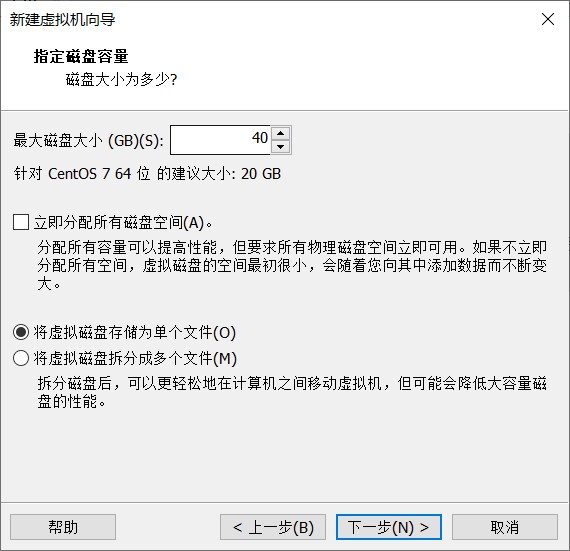
\includegraphics[width=8cm,height=6cm]{./figures/图片20.png}
\end{figure}
\end{frame}

\begin{frame}
\frametitle{系统安装}
点击【下一步(N)】后,进入指定磁盘文件页面,设置虚拟镜像文件名称,可以使用默认文件名Linux\_CentOS.vmdk,点击【下一步(N)】按钮
\begin{figure}
 %\small
 \centering
 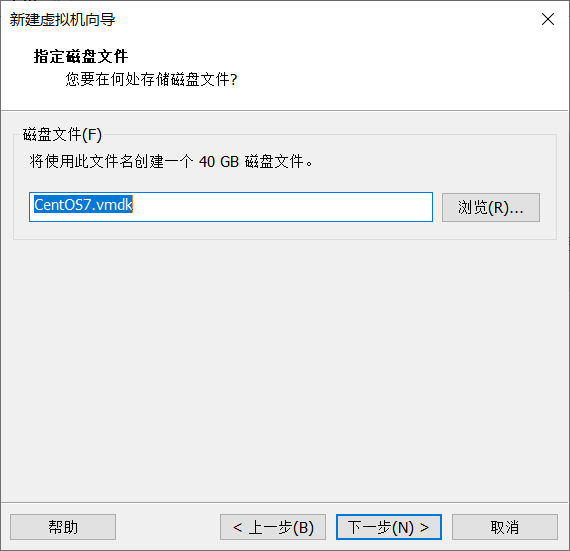
\includegraphics[width=8cm,height=6cm]{./figures/图片21.png}
\end{figure}
\end{frame}

\begin{frame}
\frametitle{系统安装}
进入虚拟机准备完成页面,创建完成,确认虚拟机信息,点击【完成】即可
\begin{figure}
 %\small
 \centering
 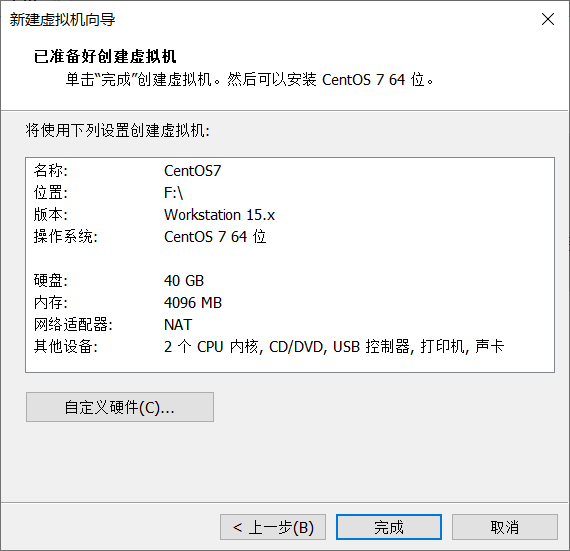
\includegraphics[width=8cm,height=6cm]{./figures/图片22.png}
\end{figure}
\end{frame}

\begin{frame}
\frametitle{系统安装}
选择“虚拟机--->设置”,进入虚拟机设置页面。选中【CD/DVD(IDE)】项,右侧选择【使用ISO映像文件(H)】,点击【浏览】按钮,选则我们下载好iso镜像文件,然后点击【确定】按钮
\begin{figure}
 %\small
 \centering
 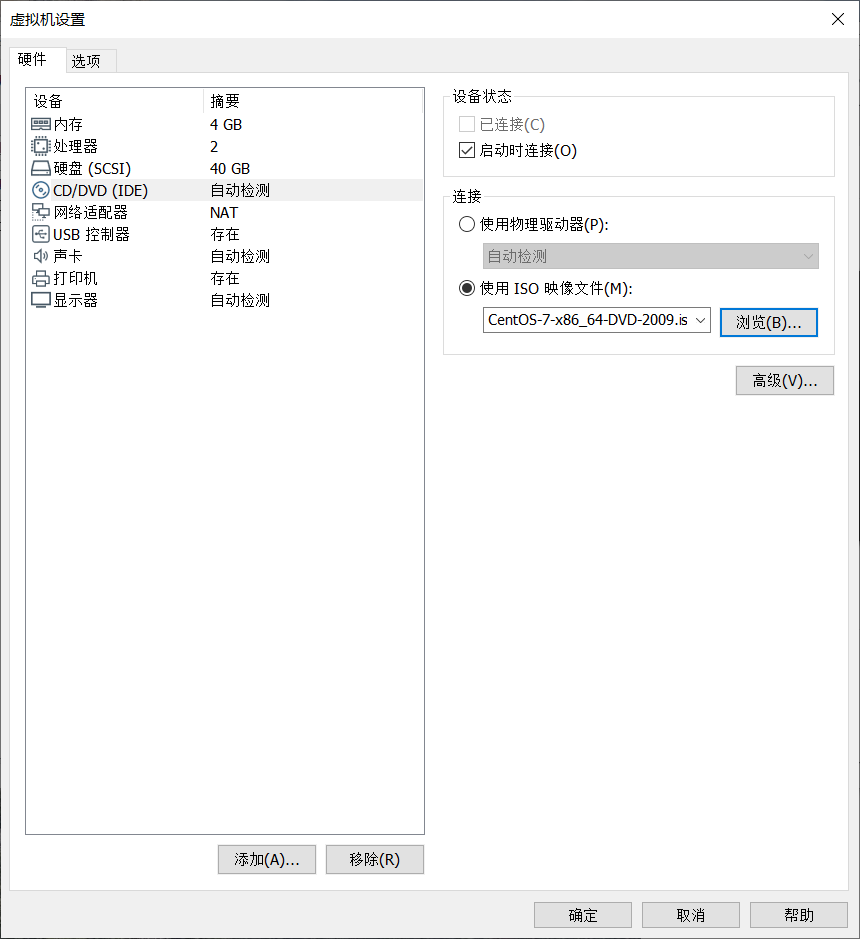
\includegraphics[width=8cm,height=6cm]{./figures/图片23.png}
\end{figure}
\end{frame}

\begin{frame}
\frametitle{系统安装}
点击【开启此虚拟机】,启动此虚拟机
\begin{figure}
 %\small
 \centering
 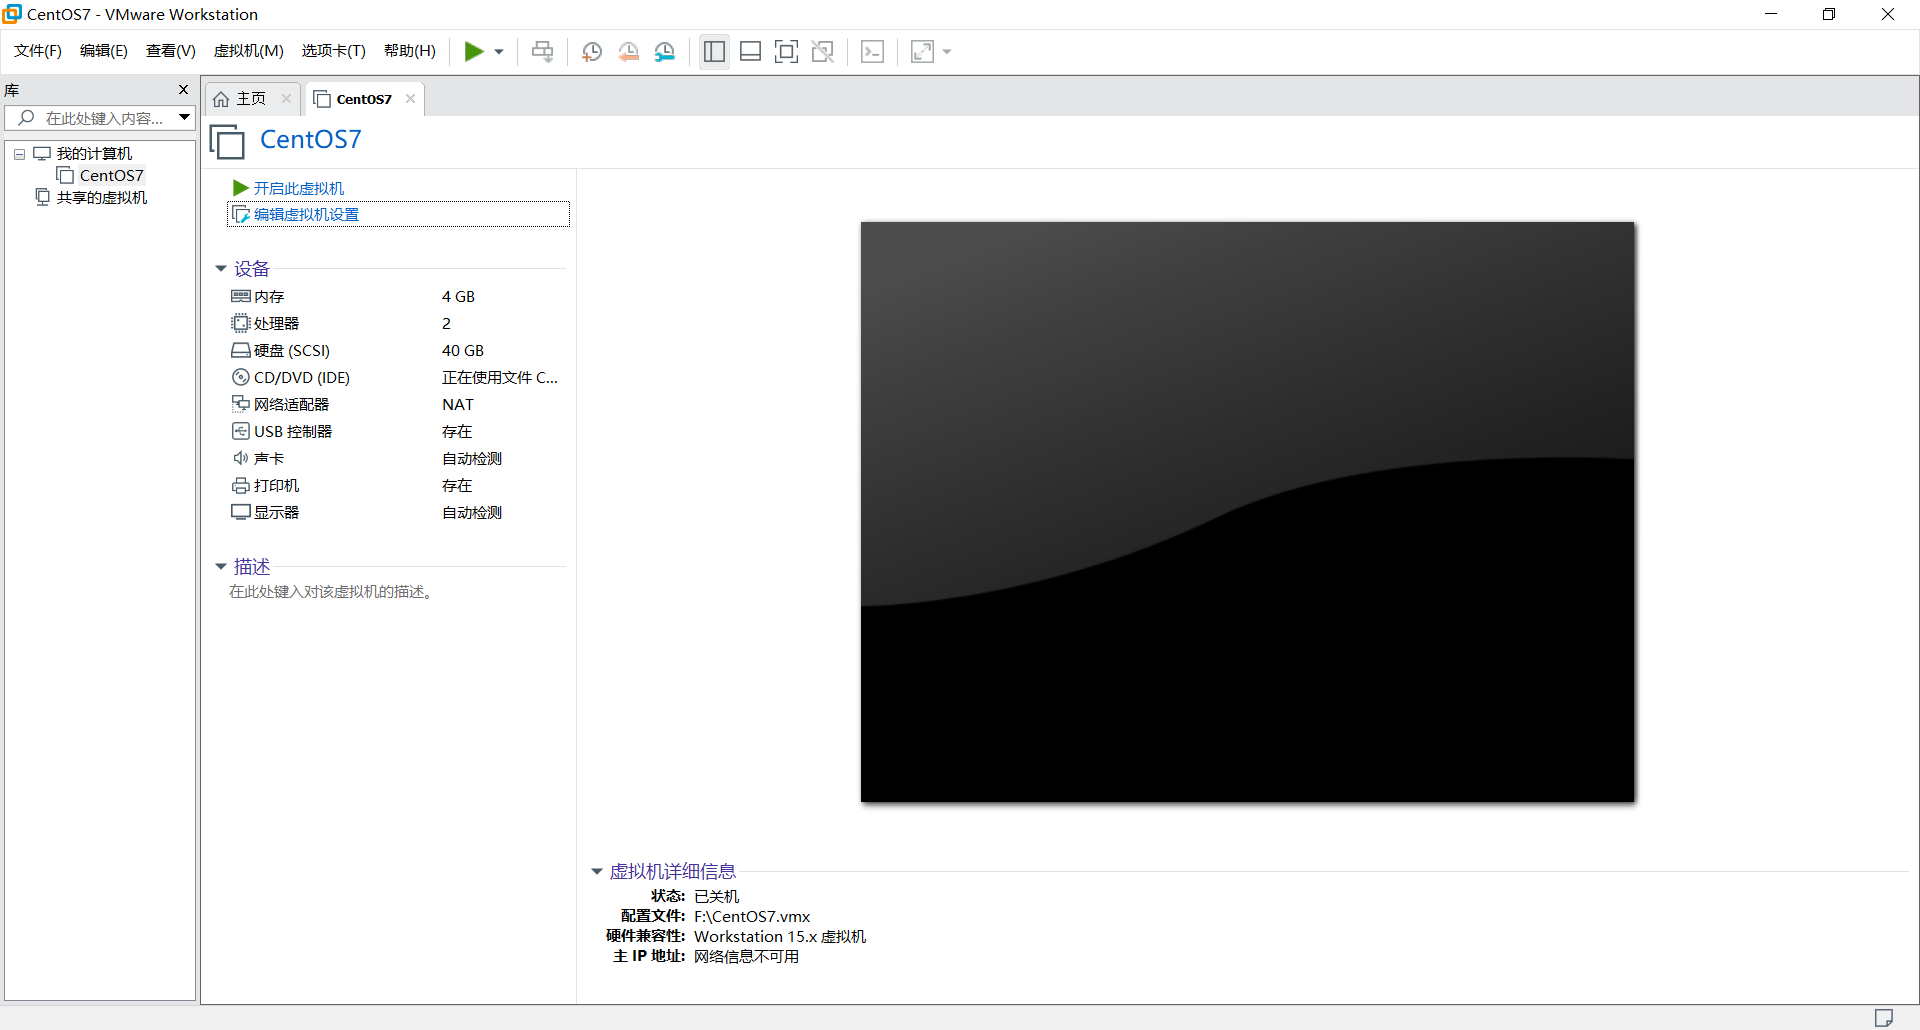
\includegraphics[width=8cm,height=6cm]{./figures/图片24.png}
\end{figure}
\end{frame}

\subsection{双系统安装}
\begin{frame}
\frametitle{双系统安装}
参考网址:https://www.cnblogs.com/masbay/p/10745170.html
    \begin{itemize}
    \item 下载rufus镜像制作软件 \\github.com/pbatard/rufus
	\item 从ubuntu官网上下载最新LTS版本20.04
	\item 装上u盘制作ubuntu启动盘
	\item 硬盘分区
	\item 进入bios界面,修改安全模式为AHCI(dell是f12,华硕、联想是f2)
	\item 将bios设为UEFI
	\item 在advanced上选择enable
	\end{itemize}

\textcolor{red}{注意:可能需要禁用显卡,请自己百度}
	
\end{frame}


\subsection{CentOS安装}

\begin{frame}
\frametitle{设置语言}
点击【开启此虚拟机】,启动此虚拟机,第一次开启虚拟机,进入CentOS Linux 7语言设置页面,选择【简体中文(中国)】,点击【继续】按钮
\begin{figure}
 %\small
 \centering
 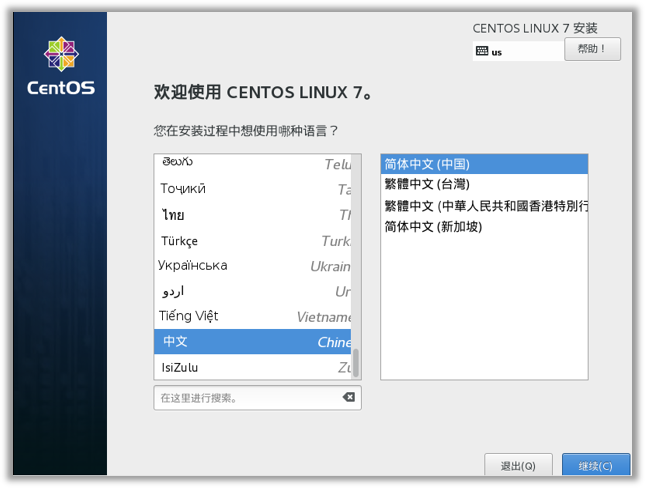
\includegraphics[width=8cm,height=6cm]{./figures/图片25.png}
\end{figure}
\end{frame}

\begin{frame}
\frametitle{软件选择}
进入软件选择界面,选择【开发及生成工作站】,点击【完成(D)】
\begin{figure}
 %\small
 \centering
 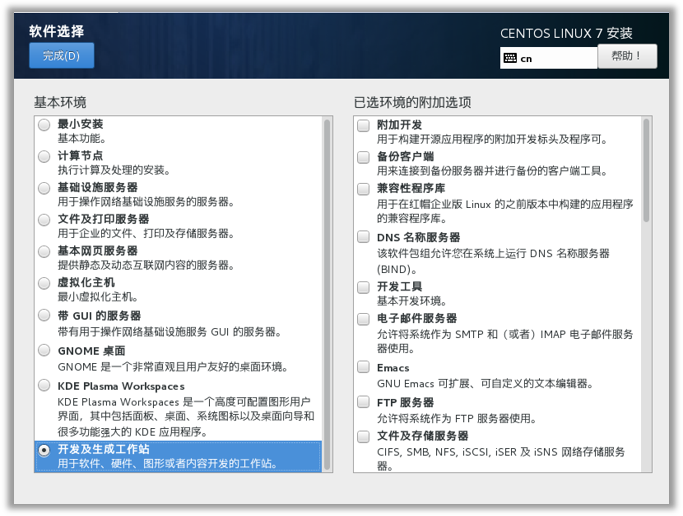
\includegraphics[width=8cm,height=6cm]{./figures/图片26.png}
\end{figure}
\end{frame}

\begin{frame}
\frametitle{安装位置}
进入CentOS7安装主界面,点击【安装位置(D)】选项
\begin{figure}
 %\small
 \centering
 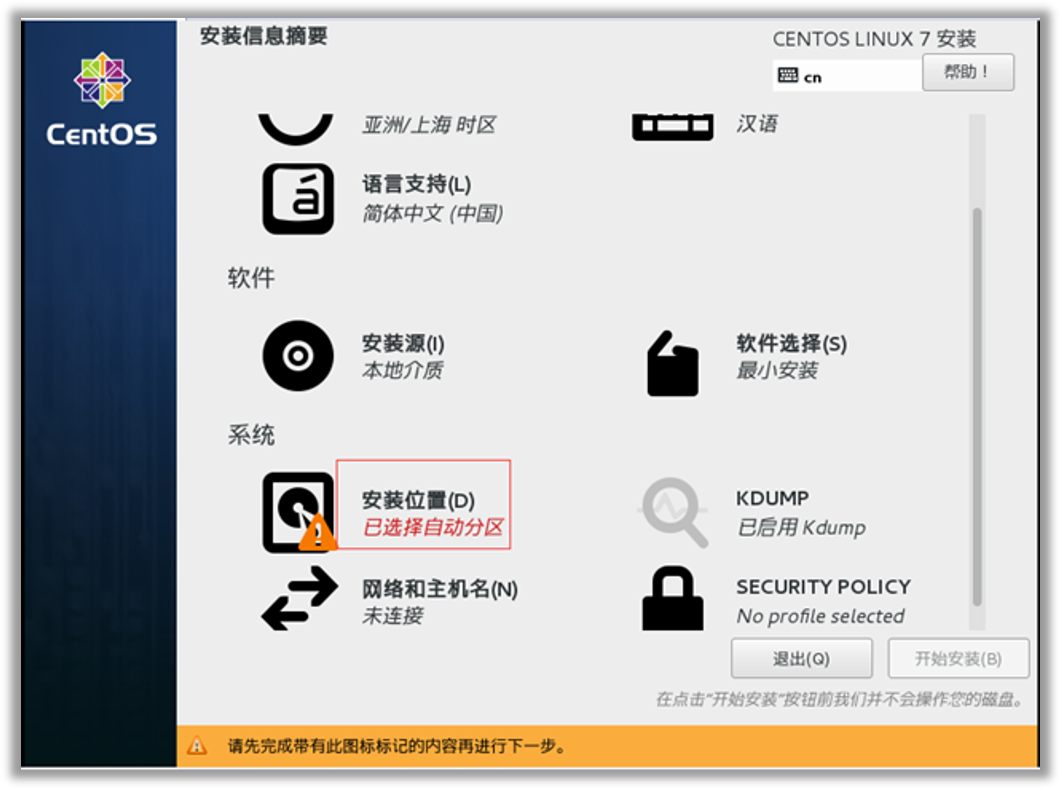
\includegraphics[width=8cm,height=6cm]{./figures/图片27.png}
\end{figure}
\end{frame}


\begin{frame}
\frametitle{分区页面}
建议选择【自动配置分区(U)】,会根据系统使用情况分配内存,点击【完成】按钮
\begin{figure}
 %\small
 \centering
 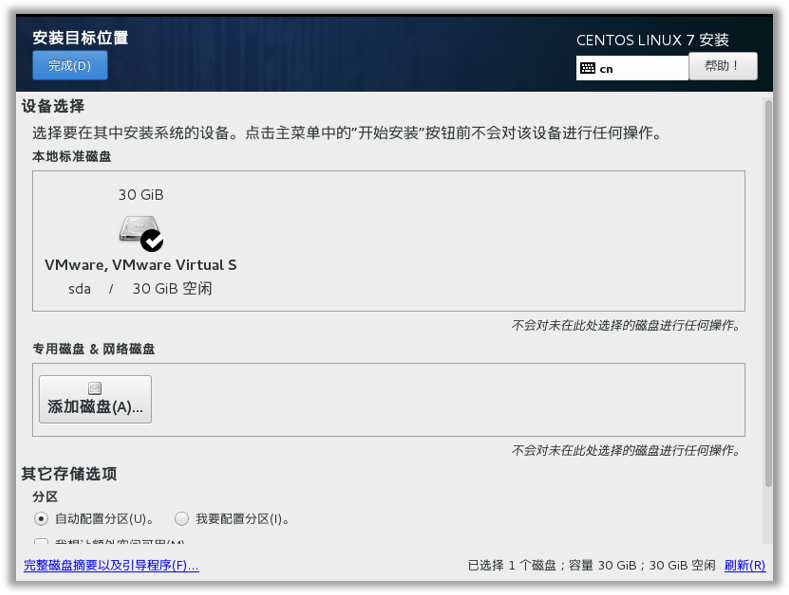
\includegraphics[width=8cm,height=6cm]{./figures/图片28.png}
\end{figure}
\end{frame}

\begin{frame}
\frametitle{网络配置}
点击【网络与主机名】选项,进入配置网络页面
\begin{figure}
 %\small
 \centering
 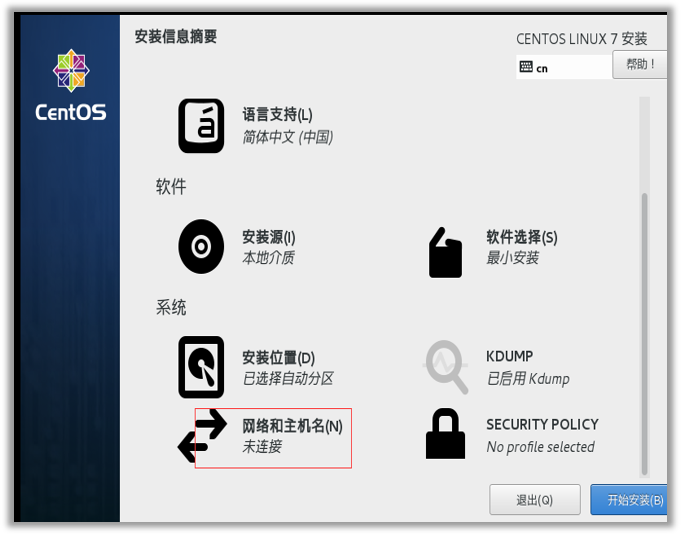
\includegraphics[width=8cm,height=6cm]{./figures/图片29.png}
\end{figure}
\end{frame}

\begin{frame}
\frametitle{网络配置}
点击以太网(ens33),进行【开启】,点击【配置】,方法(M)选择自动(DHCP),然后确定。显示【有线ens33已连接】
\begin{figure}
 %\small
 \centering
 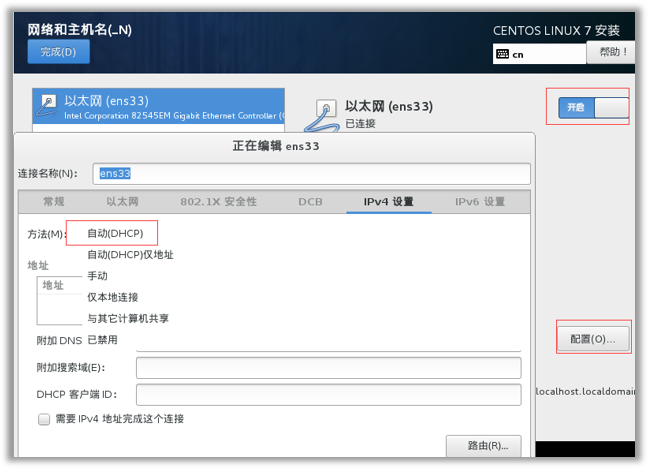
\includegraphics[width=8cm,height=6cm]{./figures/图片30.png}
\end{figure}
\end{frame}

\begin{frame}
\frametitle{开始安装}
点击【开始安装(B)】,进入安装配置界面
\begin{figure}
 %\small
 \centering
 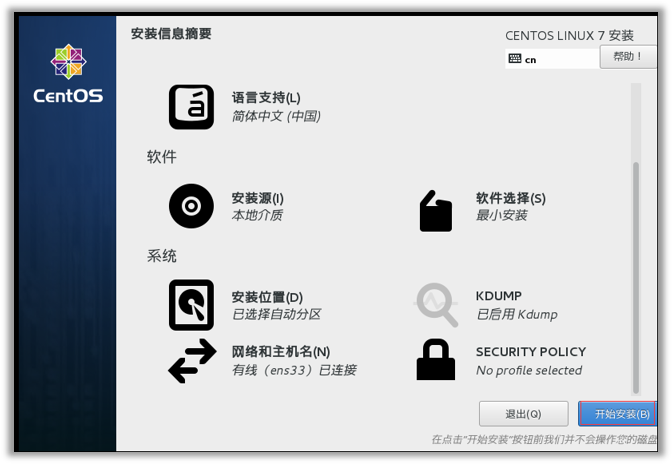
\includegraphics[width=8cm,height=6cm]{./figures/图片31.png}
\end{figure}
\end{frame}

\begin{frame}
\frametitle{密码设置}
点击【ROOT密码】选项,设置ROOT用户的密码
\begin{figure}
 %\small
 \centering
 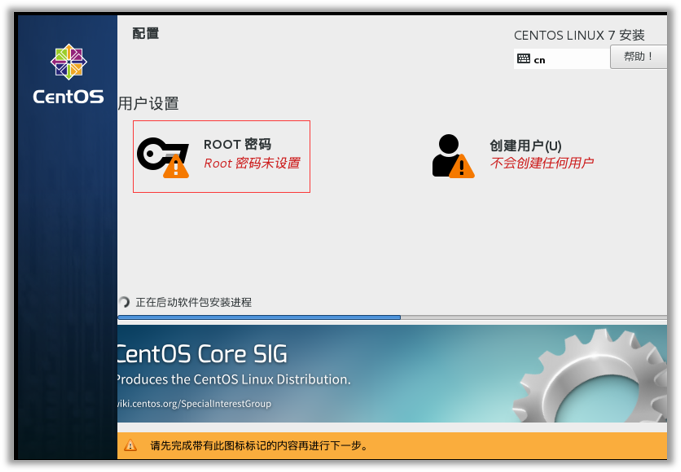
\includegraphics[width=8cm,height=6cm]{./figures/图片32.png}
\end{figure}
\end{frame}

\begin{frame}
\frametitle{设置密码}
进入设置密码界面 ,【Root密码(R)】为用户账户密码(123),【确认(C)】输入一个相同的密码,点击【完成(D)】按钮(按两次完成)
\begin{figure}
 %\small
 \centering
 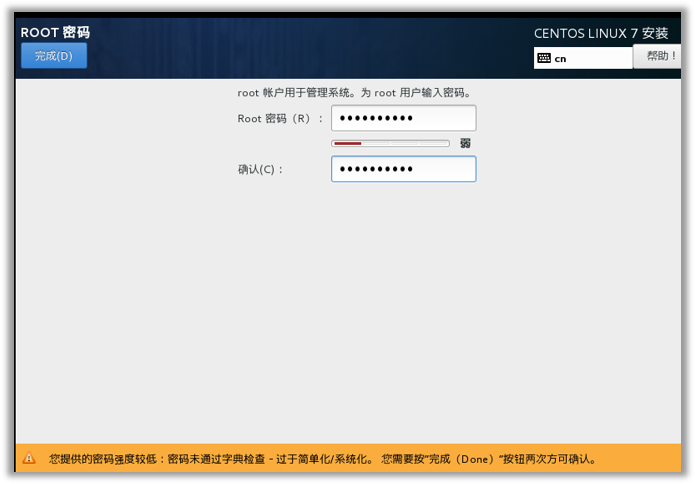
\includegraphics[width=8cm,height=6cm]{./figures/图片33.png}
\end{figure}
\end{frame}

\begin{frame}
\frametitle{设置密码}
进入安装配置显示进程的页面,点击【创建用户】选项
\begin{figure}
 %\small
 \centering
 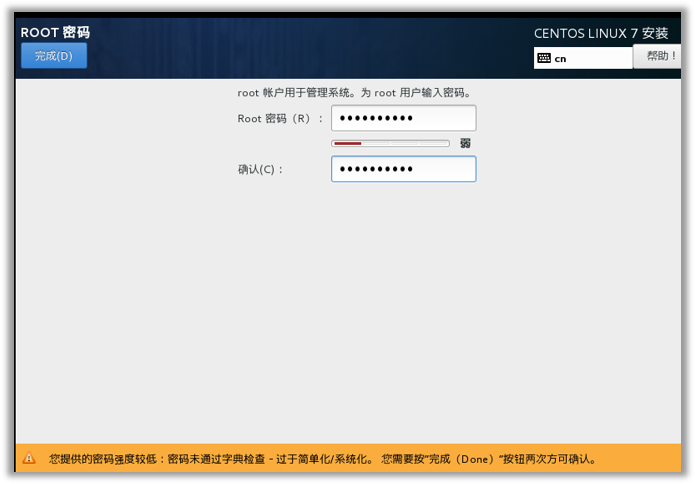
\includegraphics[width=8cm,height=6cm]{./figures/图片33.png}
\end{figure}
\end{frame}

\begin{frame}
\frametitle{创建账户}
进入新用户创建页面,为虚拟机创建其它账户。输入用户名密码,完成创建
\begin{figure}
 %\small
 \centering
 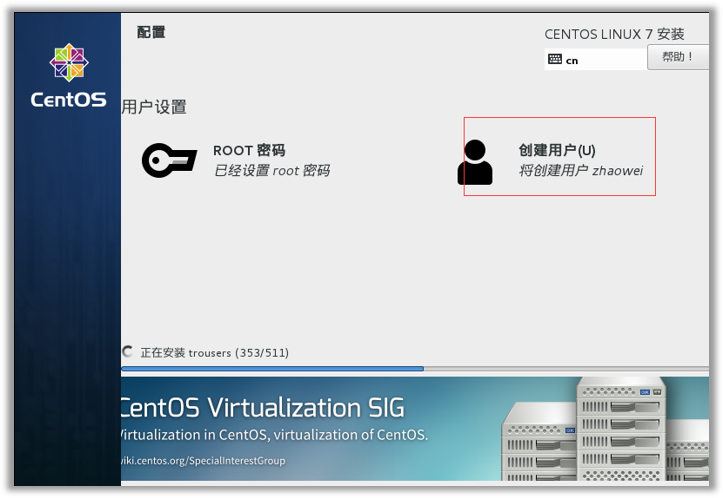
\includegraphics[width=8cm,height=6cm]{./figures/图片34.png}
\end{figure}
\end{frame}

\begin{frame}
\frametitle{成功安装}
配置完成后,点击【重启(R)】按钮,输入用户名密码,显示下面图形化页面,说明CentOS系统安装成功
\begin{figure}
 %\small
 \centering
 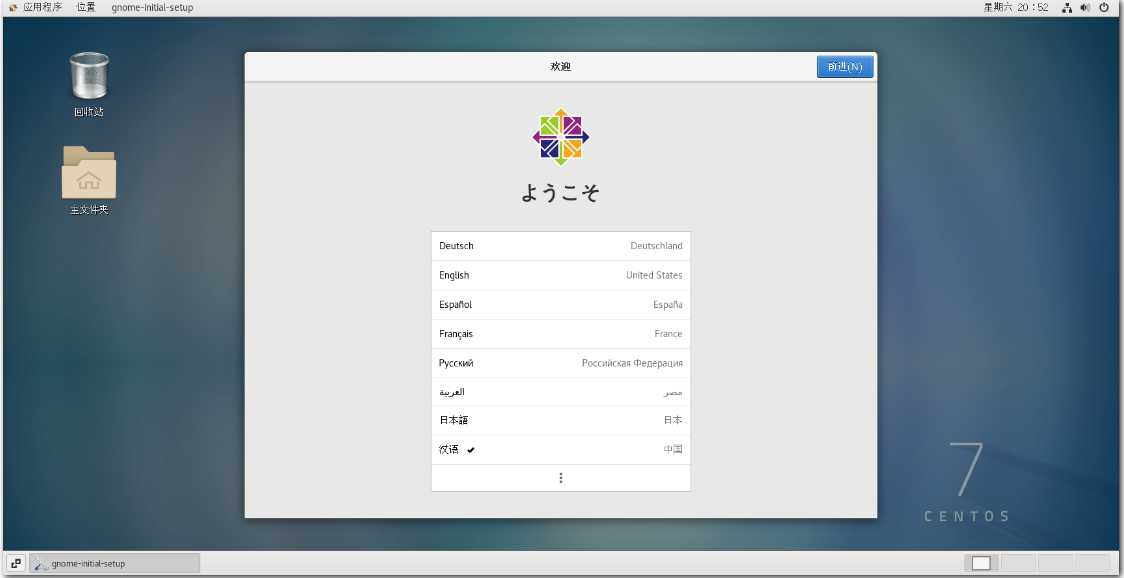
\includegraphics[width=8cm,height=6cm]{./figures/图片35.png}
\end{figure}
\end{frame}

\section{常用命令}
\begin{frame}
\frametitle{命令查询网址}
\begin{itemize}
\item https://www.runoob.com/linux/linux-command-manual.html
\item https://www.linuxcool.com/
\item https://coolshell.cn/articles/5426.html
\end{itemize}
\end{frame}

\begin{frame}
\frametitle{基本格式}
command [-options] parameter1 parameter2 ...
一行命令中第一个输入的部分绝对是『命令(command)』或『可运行文件案』
\begin{itemize}
\item command 为命令的名称,例如变换路径的命令为cd 等等;
\item [] 并不存在于实际的命令中,而加入选项配置时,通常选项前会带- 号,例如-h;有时候会使用选
项的完整全名,则选项前带有– 符号,例如–help;
\item parameter1 parameter2.. 为依附在选项后面的参数,或者是command 的参数;
\item 命令, 选项, 参数等这几个咚咚中间以空格来区分,不论空几格shell 都视为一格;
\item 命令太长的时候,可以使用反斜杠(n) 来跳脱[Enter] 符号,使命令连续到下一行。注意!反斜杠后就立
刻接特殊字符,才能跳脱!
\item 在Linux 系统中,英文大小写字母是不一样的。举例来说,cd 与CD 并不同。

在命令行里执行语句主要有两种情况,一种是会直接显示结果回到命令提示符等待下一个命令输入,另一个是
进入命令的环境直到结束该命令才回到命令提示符的环境。
\end{itemize}
\end{frame}

\begin{frame}
\frametitle{关机、重启}
\begin{itemize}
\item reboot
\item poweroff、halt、shutdown -h
\end{itemize}
\end{frame}

\begin{frame}
\frametitle{常用热键}
\begin{itemize}
\item Tab 补全命令和文件补齐
\item ctrl+c 中断目前程序
\item ctrl+d 键盘输入结束(相当于输入exit)
\end{itemize}
\end{frame}

\begin{frame}
\frametitle{文件命令}
\begin{itemize}
\item cd 切换目录,pwd 显示当前目录,mkdir 新建一个新的目录,rmdir 删除一个空目录
\item . 此层目录,.. 上一层目录,-前一个工作目录,̃ 目前用户所在的主文件夹
\item pwd 显示绝对路径
\item rm -r 删除目录下所有文件,* 为通配符,-i 互动删除会先询问
\item ls -a 列出全部文件包括隐藏文件,-d 仅列出目录本身,-l 列出长数据串(包括文件属性和权限)
\end{itemize}
\end{frame}

\begin{frame}
\frametitle{文件命令}
\begin{itemize}
\item cp -s 复制成快捷方式,-r 递归的持续复制用于目录复制,-p 连用文件的属性一起复制过去,-i 若目标文件已经存在覆盖时会询问操作的进行,-d 若源文件为接文件这复制链接文件属性,-a 相当于-pdr
\item mv -f 若果目标已经不会询问直接覆盖,-i 已经存在时会询问
\item cat -n 现实文档内容会列出行号空白行也会有行号
\item ln -s [要创建的文件或文件夹] [软链接存放位置]\\建立软连接
\item ln [要创建的文件或文件夹] [软链接存放位置]\\建立硬连接
\end{itemize}
\end{frame}


\begin{frame}
\frametitle{压缩和解压}
\begin{itemize}
\item zip\\压缩zip  target\_filename  source\_filenames\\解压unzip filename.zip
\item tar.gz\\压缩tar -czvf test.tar.gz a.txt   //压缩 a.txt文件为test.tar.gz\\解压tar -xzvf test.tar.gz
\end{itemize}
\end{frame}

\section{Vim常用命令}
\begin{frame}
\frametitle{Vim常用命令}
\begin{itemize}
\item vim 文件名
\\打开文件 
\item :wq
\\保存并退出文件
\item :e!
\\放弃修改,编辑区回复原样
\end{itemize}
\end{frame}

\section{小任务}
\begin{frame}
\frametitle{小任务}
\begin{itemize}
\item 在/home/Documents下创建一个a.txt
\\touch
\item 在/home/Documents下创建一个文件夹test
\\mkdir
\item 移动a.txt到test里面
\\mv
\item 编辑a.txt,输入Linux and vim,保存退出
\\vi
\item 查看文件
\\cat
\item 删除整个test文件夹(包括里面的a.txt)
\\rm
\end{itemize}
\end{frame}

\begin{frame}
\begin{center}
\Huge \textcolor{red}{谢~~谢~~大~~家!}
\end{center}
\end{frame}

\end{document}
